\chapter{1D Boundary Value Problem}
\section*{Introduction}
The first homework assignment is concerned with solving 1D boundary value problems using the finite element method. The main purpose it to introduce the ''mFEM'' library that will be used throughout this course and to which will be expaned upon for each assignment. The mFEM library is an object-oriented set of code designed for this course. If you are not familiar with object-oriented programming in general or with MATLAB refer to the folowing online documentation. 
\begin{center}
\href{http://www.mathworks.com/discovery/object-oriented-programming.html}{www.mathworks.com/discovery/object-oriented-programming.html}
\end{center}

\section*{mFEM Installation}
Before the mFEM library is ready to use, it must be installed, this is accomplished by following these simple steps.
\begin{enumerate}
\item Change the current folder in MATLAB to the folder containing this file, i.e. the folder to which you unzipped the contents of the assignment.
\item Run the install script:
\begin{lstlisting}
install;
\end{lstlisting} 
\end{enumerate}
\section*{mFEM Documentation}
The mFEM documentation will be available from the MATLAB helpbrowser after the \texttt{install} function has been executed. To access the mFEM documentation:
\begin{enumerate}
\item Open the help browser by typing \texttt{doc} into the command line or selecting the help icon. 
\item Then search for ``mFEM,'' this will open the main documentation page for the library.
\end{enumerate}

\section*{Tutorial Problem}
Before completing this homework, review the tutorial program (\texttt{tutorial.m}) (a link to the detailed documentation is available in the mFEM documentation), which solves the following problem.

Consider a bar with a uniformly distributed heat source ($s$) of 5 W/m. The bar has a uniform cross sectional area ($A$) of 0.1 m$^2$ and thermal conductivity ($k$) of 2 W/(\C m). The length of the bar is 4 m. The boundary conditions are $T(0) = 0$ \C ~and $q(4) = 5$ W/m$^2$ as shown in the figure below. 

\begin{center}
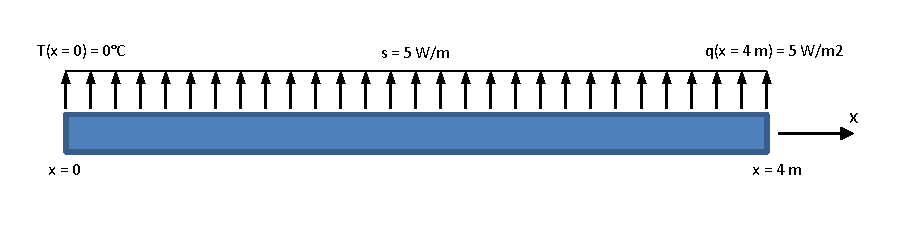
\includegraphics{HW2/tutorial.pdf}
\end{center}

\question{HW2-1}
\question{HW2-2}
\question{HW2-3}
\question{HW2-4}





